\section{Results and Analysis} \label{sec:results}
% 1. Accuracy (F1 + MCC) auf SICK und eSNLI einzeln nach Kategorien
% 2. Auf Bias überprüfen: Vergleich vom Modell für wichtig erachtete Token mit von Menschen als wichitg erachtete Tokens
% Visualisierungen:
% - Confusion Matrix (Gentrennt nach Phänomenen)
% - Tabellen Interpretability Metriken (siehe ferret)
In this section the results of our experiments are described and thoroughly analyzed. The results are grouped according to the hypotheses they support.

\subsection{Testing H1}

\begin{table}[ht!]
    \centering
    \caption{Prediction performance when using prompting with different word groups on the \acs{SICK} dataset. The best result is shown in \textbf{bold} and the second-best is \underline{underlined}.}
    \begin{tabular}{l c c}
        \toprule
        \multicolumn{1}{c}{Word Group} & \acs{MCC} & $\text{F}_1$ \\
        \midrule
        A Priori & $\underline{25.51}\%$ & $\mathbf{54.31\%}$ \\
        Simple & $20.56\%$ & $\underline{34.40\%}$ \\
        Tuned & $\mathbf{29.11\%}$ & $34.08\%$ \\
        \bottomrule
    \end{tabular}
\end{table}

\subsection{Testing H2}
Figure~\ref{fig:ferret-sample} shows the explanations for the finetuned model's classification of a sample from the validation split of the \ac{e-SNLI} dataset obtained using ferret \cite{ferret}. It can be seen that the meaning of the quantifiers in this sample is not considered by the model: The usage of quantifiers in this sample makes it a contradiction but the model attaches high importance only to the quantifier \enquote{all} whereas \enquote{several} has very low importance to the model. The existence of such samples where the model only poorly captures the importance of quantifiers shows that the model is biased after fine-tuning on \ac{MultiNLI}.

\begin{figure*}[h!]
    \centering
    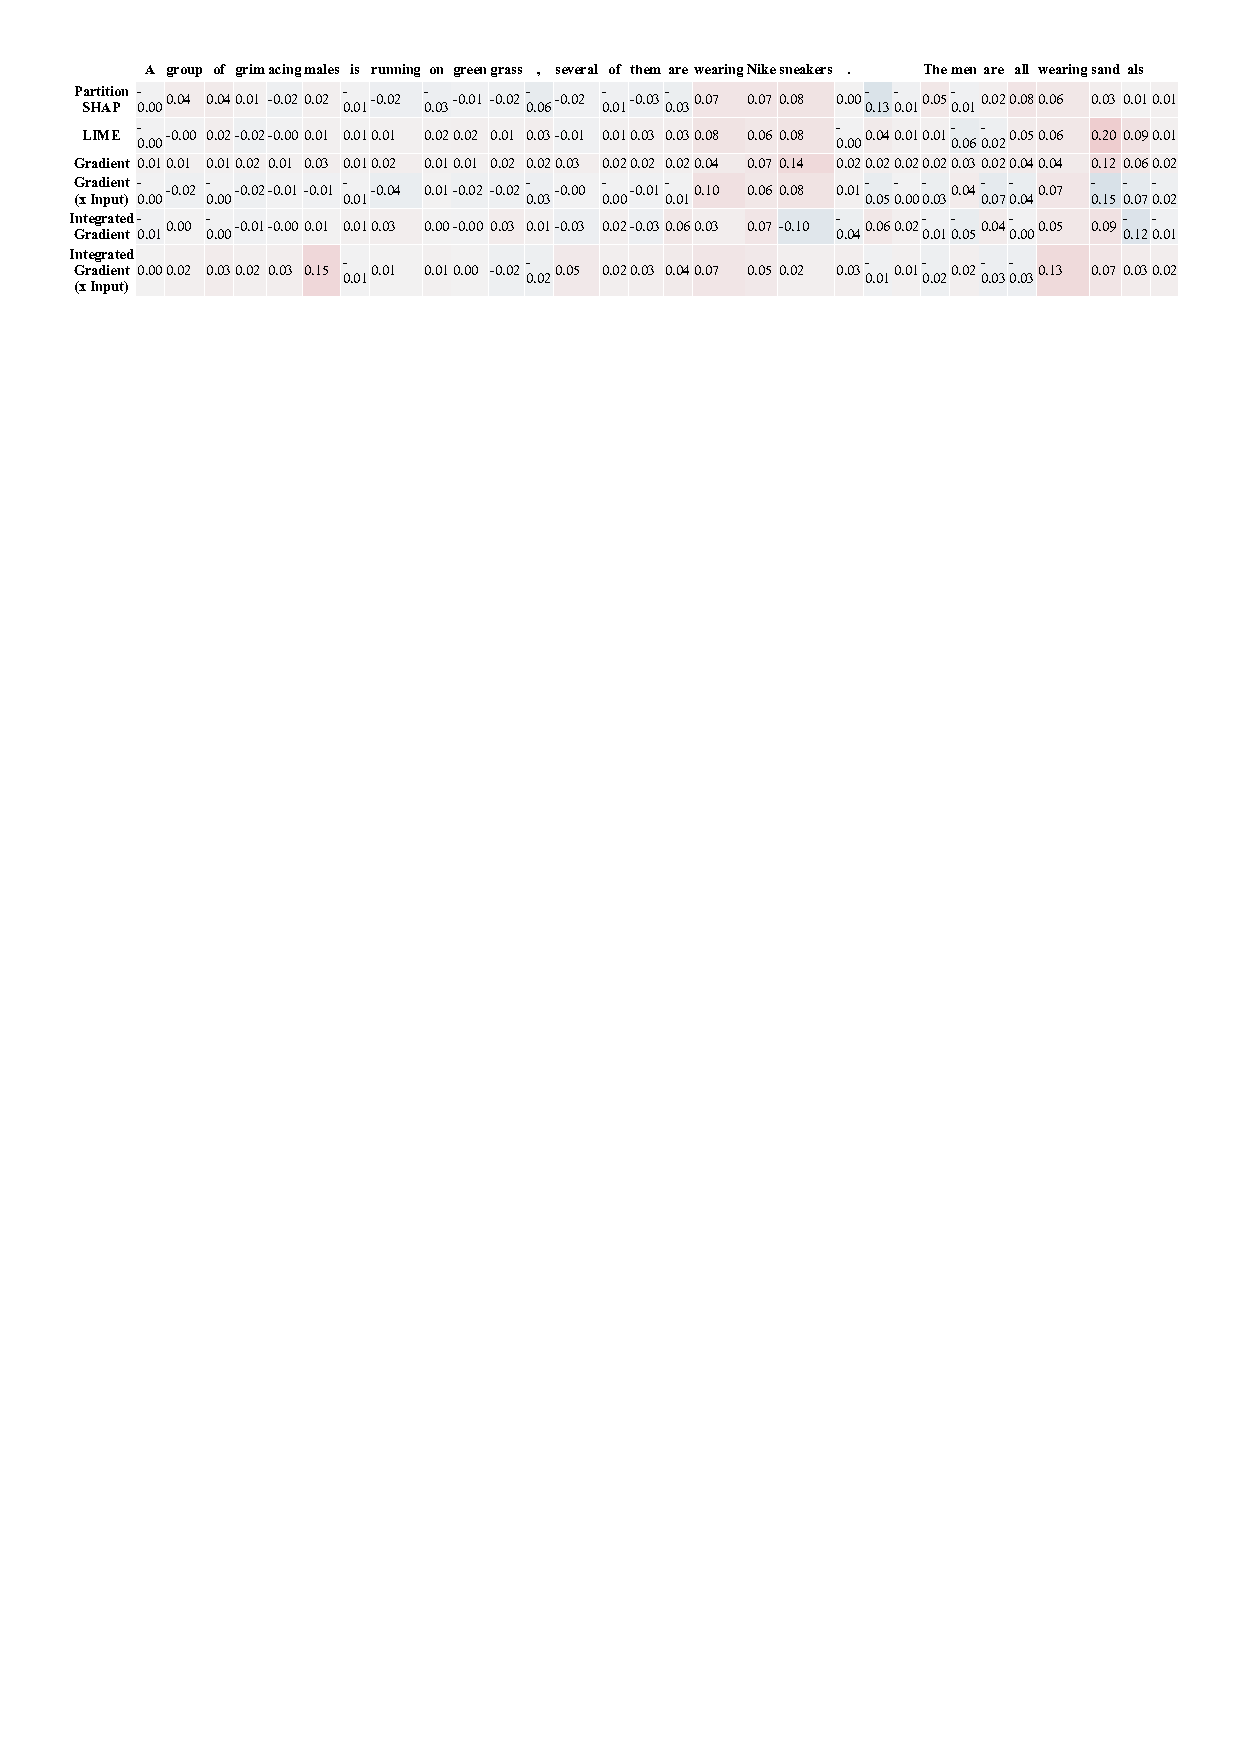
\includegraphics[width=\textwidth]{./images/ferret_sample.pdf}
    \caption{Expamle of a bad explanation}
    \label{fig:ferret-sample}
\end{figure*}

\subsection{Testing H3}

\begin{table}[ht!]
    \centering
    \caption{Prediction performance of our fine-tuned models on the \acs{SICK} dataset. The best result is shown in \textbf{bold} and the second-best is \underline{underlined}.}
    \begin{tabular}{l c c}
        \toprule
        \multicolumn{1}{c}{Model} & \acs{MCC} & $\text{F}_1$ \\
        \midrule
        Base & $49.49\%$ & $56.60\%$ \\
        Hypothesis-Only\tablefootnote{Average of three runs with different seeds} & $14.13\%$ & $40.02\%$ \\
        Filtered $2/3$ & $46.21\%$ & $54.12\%$ \\
        Filtered $2/3$ longer & $36.17\%$ & $52.85\%$ \\
        Filtered $3/3$ & $48.73\%$ & $56.94\%$ \\
        Filtered $3/3$ longer & $\mathbf{52.31\%}$ & $\mathbf{62.04\%}$ \\
        Ensembled & $\underline{51.65\%}$ & $\underline{59.88\%}$ \\
        Recast & n/a & n/a \\
        \bottomrule
    \end{tabular}
    \label{tab:res:finetuned}
\end{table}

\subsection{Testing H4}
To test this hypothesis, we trained multiple models and evaluated their predictive performance in general and further analyzed the best model. The predictive performance of all models can be seen in \autoref{tab:res:finetuned}, the names follow the names of the datasets introduced in \autoref{sec:experiments}. In this case, a high correlation between the F$_1$-Score and \ac{MCC} can be seen, so we do not need to consult additional metrics. The differences in \ac{MCC} are bigger and the \ac{MCC} was more meaningful when comparing the results of the different prompting methods, therefore we mainly analyze the \ac{MCC} scores.

Unexpectedly, the filtered models perform worse than the base fine-tuned model, even though the data quality should be better. As the models trained on the filtered datasets have been trained for fewer iterations in three epochs, we interpret the inferior results as being because of less training. When evaluating the models trained for more epochs, we can see an improvement for \enquote{Filtered 3/3} and deterioration for \enquote{Filtered 2/3}. This result is only slightly unexpected and can be attributed to \enquote{Filtered 2/3} being more harshly filtered and therefore have even fewer samples which cannot be balanced out by the higher data quality of filtering biased samples more easily. \enquote{Filtered 3/3} shows better performance when trained longer, which indicates it providing a better tradeoff between data quality and data quantity. Therefore, we further analyze \enquote{Filtered 3/3} and use it to compare to the ensembled model.

The ensemble model performs better than the baseline and slightly worse than the filtered model trained longer. This indicates that bias is successfully mitigated during training, as predictive performance on the less biased out-of-domain evaluation set is improved. The performance is still slightly better for the filtered model, we further analyze that instead of the ensemble.

\begin{figure}[ht]
    \centering
    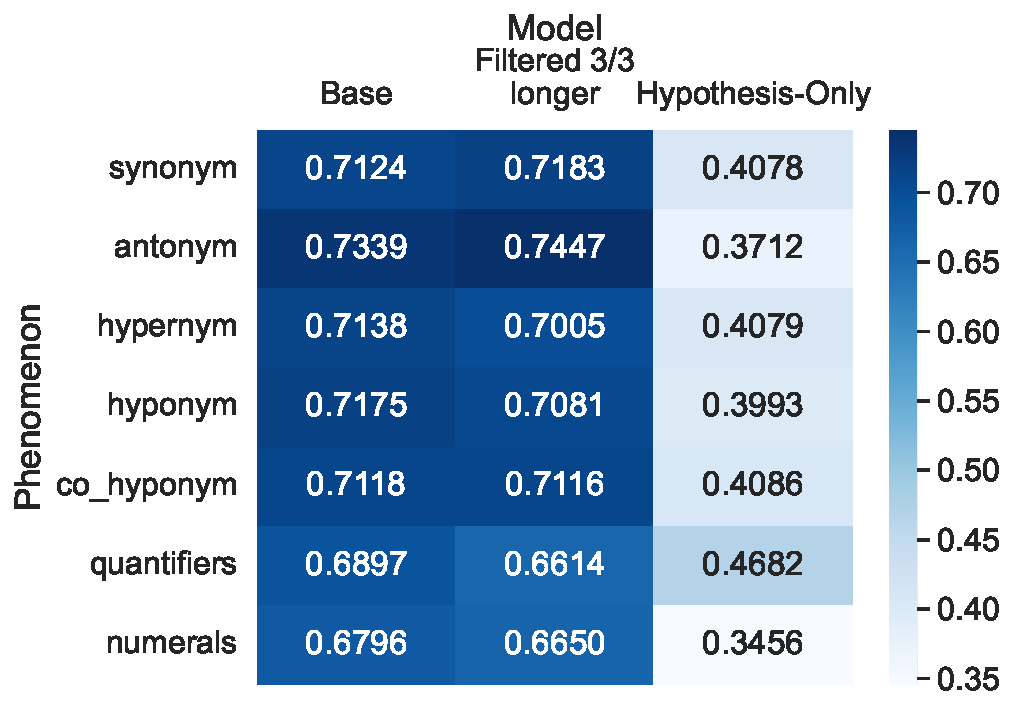
\includegraphics[width=0.9\columnwidth]{./images/metric_heatmaps_phenomena/all_words/matthews_correlation.pdf}
    \caption{\ac{MCC} scores for the models trained on different datasets separated by linguistic phenomena}
    \label{fig:metric-heatmap-phenomena-mcc}
\end{figure}

Figure~\ref{fig:metric-heatmap-phenomena-mcc} depicts the \ac{MCC} scores separated by linguistic phenomena for the filtered model compared to the base fine-tuned model. We can see slightly improved performance for antonyms with harshly decreased performance for quantifiers and similar performance for all other phenomena. The decreased performance for quantifiers can be explained by the hypothesis-only model being more accurate on quantifiers and therefore more examples of quantifiers being discarded as biased during filtering. The decreased performance might be explained by either fewer samples of this phenomenon existing after filtering or the evaluation set having the same biases as the training set and thus decreased performance for it that would not exist for a less biased dataset. The increased performance on antonyms but decreased performance on numerals is surprising, as both have poor prediction performance for the hypothesis-only model and thus should not be filtered too much. We interpret that result as random noise or just a general decrease in bias that is randomly effective for antonyms but is not for numerals. Nonetheless, the filtering is beneficial for overall prediction performance, which can be explained by samples not being detected as part of any of our phenomena.

% TODO: description of bias plots

\subsection{Testing H5}